\subsection{\acf*{SVM}}
\label{sec:svm}

\acfp{SVM} were initially proposed by Wladimir Wapnik and Aleksei Tscherwonenkis in 1974 \cite{vapnik1974theory}. They showed a method for classification and linear regression, which becomes one of the most popular algorithms in the field of artificial intelligence \cite{russellnorvig-ai}. A \ac{SVM} is typically a binary classifier, which separates multiple datapoints into two classes. A supervised \ac{SVM} training is done by placing a line (for 2-D dimensional data) or a hyperplane between two different classes by maximizing the margin between all datapoints (as one can see in \figref{svm_lin}). Other algorithms may produce a linear separation by one of the lines in \figref{svm_lin:hyp}, which would always be a correct classification of the given data. Nevertheless, especially the lines near to datapoints of one class will fail if a new datapoint has to be classified, which belongs to this class, but would be on the wrong side of the line. \acp{SVM} on the other hand try to minimize this generalization loss instead of the empirical loss by choosing a line, which has the maximum margin to the separated datapoints as shown in \figref{svm_lin:maxmarg}.

\begin{figure}
\begin{subfigure}[t]{0.5\linewidth}
\centering
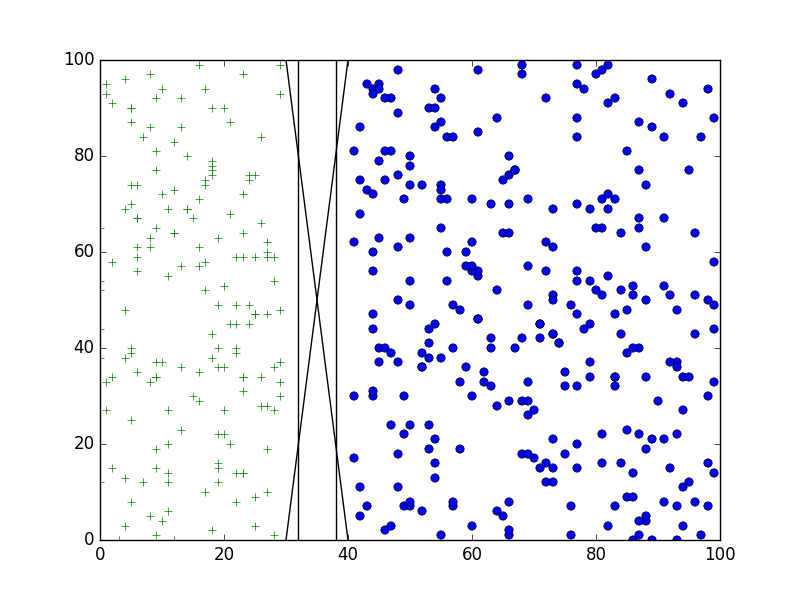
\includegraphics[width=\linewidth]{images/svm_lin}
\caption{Separated by different lines.}
\label{fig:svm_lin:hyp}
\end{subfigure}%
%
\begin{subfigure}[t]{0.5\linewidth}
\centering
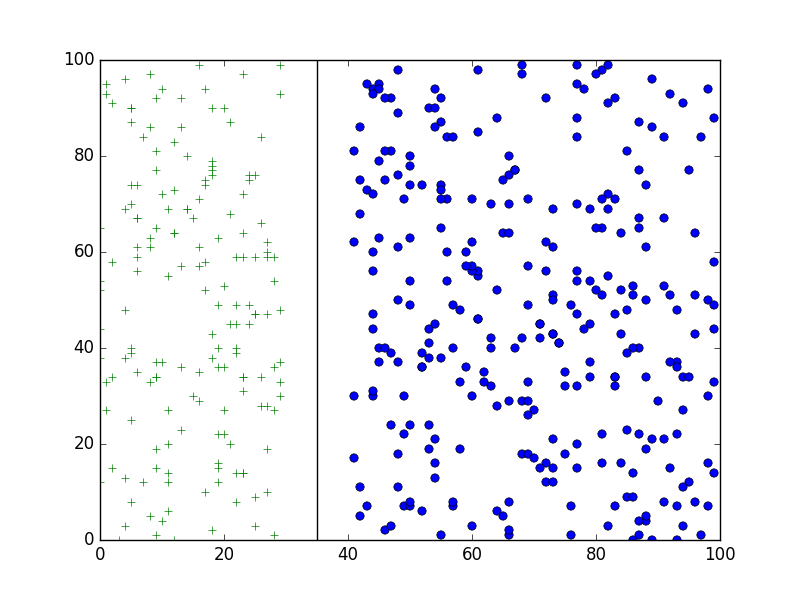
\includegraphics[width=\linewidth]{images/svm_lin_maxmarg}
\caption{Separated by a line with maximum margins.}
\label{fig:svm_lin:maxmarg}
\end{subfigure}
\caption{2 classes of datapoints, linear separable}
\label{fig:svm_lin}
\end{figure}

To find an optimal separator, the \eqnref{svm:maxmarg} with the constraints $a_j \ge 0$ and $\sum_j a_j y_j = 0$ has to be solved. This quadratic programming optimization problem can be solved by a Lagrangian and the Kuhn-Tucker theorem as described by Cortes and Vapnik \cite{cortes1995support}.

\begin{equation}
\arg\max_\alpha \sum_j \alpha_j - \frac{1}{2} \sum_{j,k} \alpha_j, \alpha_k y_j y_k (x_j \cdot x_k)
\label{eqn:svm:maxmarg}
\end{equation}

As some data is not linearly separable, it may be required to move the data into a higher dimensional space as shown in the sample images \figref{svm_nonsep}. In general a dataset of $N$ points can be linearly separated in a $N-1$ dimensional space \cite{russellnorvig-ai}.
To obtain high dimensional datapoints $x$, they will be transfered into a high dimensional feature space by $F(x)$. This means that we can replace the $x_j \cdot x_k$ with $F(x_j) \cdot F(x_k)$. A possible function $F$ for the sample could introduce an additional dimension by $F(x) \rightarrow x_1^2, x_2^2, \sqrt{2} x_1 x_2$. With this function it can be shown that

\begin{equation}
F(x_i) \cdot F(x_j) = (x_i \cdot x_j)^2
\end{equation}

The equation $(x_i \cdot x_j)^2$ is called kernel function and is often written as $k(x_i, x_j)$. This also represents the so called kernel trick, which means that all occurrences of $(x_i \cdot x_j)$ are replaced by the kernel function and therefore allow to find optimal solutions in an arbitrary high dimensional feature space. The found solution can be afterwards retransfered into the original space and result into arbitrary shapes.

As the \ac{SVM} is used to classify data into two classes, some modifications have to be applied to support multi-class data. The two most used algorithms are to train one-vs-all or one-vs-one classifiers. One-vs-all classifiers are trained for each possible class and against all other datapoints as negative set. This type of classifiers can be used to detect if a sample point is possibly part of a specific class, but they cannot express, which of the assigned classes are the most likely ones. The one-vs-one classifiers on the other hand are trained between each possible class-class combination. This enables the comparison of a sample in respect to the different classes.

\begin{figure}
\begin{subfigure}[t]{0.5\linewidth}
\centering
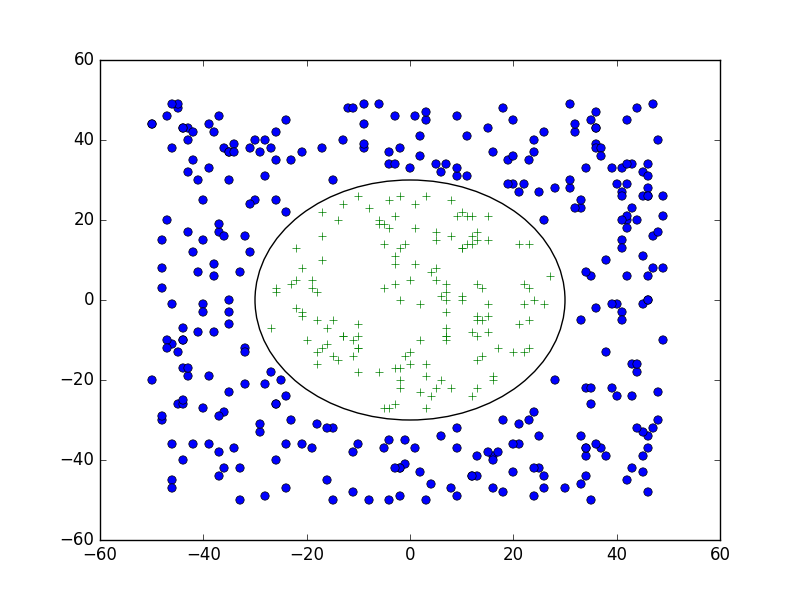
\includegraphics[width=\linewidth]{images/svm_2d}
\caption{Non-separable datapoints at a low dimensional space.}
\label{fig:svm_nonsep:2d}
\end{subfigure}%
%
\begin{subfigure}[t]{0.5\linewidth}
\centering
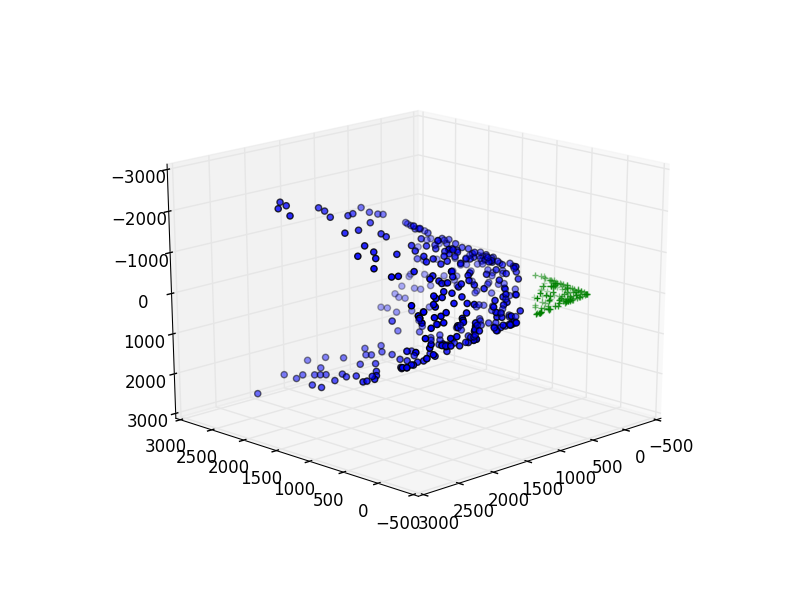
\includegraphics[width=\linewidth]{images/svm_3d}
\caption{But separable in a higher dimensional space.}
\label{fig:svm_nonsep:3d}
\end{subfigure}
\caption{Linear separation in low and high dimensional spaces.}
\label{fig:svm_nonsep}
\end{figure}

% problem
% grafik
% kernel trick
% warum
